% Created by tikzDevice version 0.12.6 on 2026-05-17 18:10:21
% !TEX encoding = UTF-8 Unicode
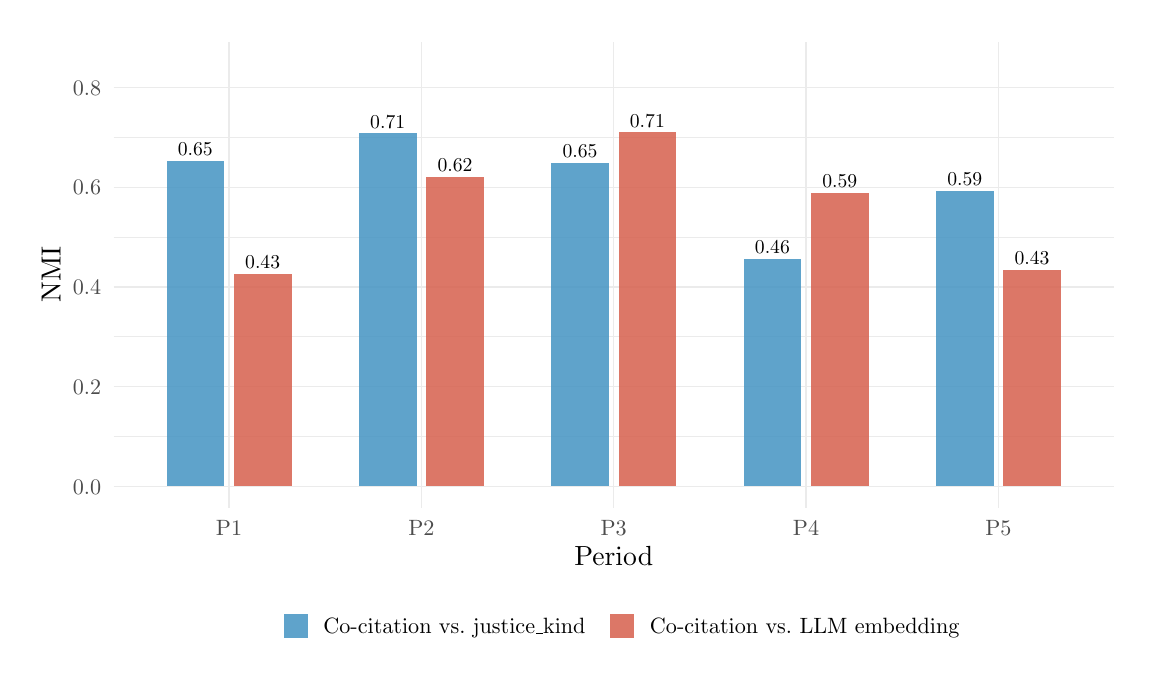
\begin{tikzpicture}[x=1pt,y=1pt]
\definecolor{fillColor}{RGB}{255,255,255}
\path[use as bounding box,fill=fillColor,fill opacity=0.00] (0,0) rectangle (397.48,231.26);
\begin{scope}
\path[clip] (  0.00,  0.00) rectangle (397.48,231.26);
\definecolor{fillColor}{RGB}{255,255,255}

\path[fill=fillColor] ( -0.00,  0.00) rectangle (397.48,231.26);
\end{scope}
\begin{scope}
\path[clip] ( 31.05, 57.85) rectangle (392.48,226.26);
\definecolor{drawColor}{gray}{0.92}

\path[draw=drawColor,line width= 0.3pt,line join=round] ( 31.05, 83.52) --
	(392.48, 83.52);

\path[draw=drawColor,line width= 0.3pt,line join=round] ( 31.05,119.54) --
	(392.48,119.54);

\path[draw=drawColor,line width= 0.3pt,line join=round] ( 31.05,155.57) --
	(392.48,155.57);

\path[draw=drawColor,line width= 0.3pt,line join=round] ( 31.05,191.59) --
	(392.48,191.59);

\path[draw=drawColor,line width= 0.5pt,line join=round] ( 31.05, 65.51) --
	(392.48, 65.51);

\path[draw=drawColor,line width= 0.5pt,line join=round] ( 31.05,101.53) --
	(392.48,101.53);

\path[draw=drawColor,line width= 0.5pt,line join=round] ( 31.05,137.56) --
	(392.48,137.56);

\path[draw=drawColor,line width= 0.5pt,line join=round] ( 31.05,173.58) --
	(392.48,173.58);

\path[draw=drawColor,line width= 0.5pt,line join=round] ( 31.05,209.60) --
	(392.48,209.60);

\path[draw=drawColor,line width= 0.5pt,line join=round] ( 72.75, 57.85) --
	( 72.75,226.26);

\path[draw=drawColor,line width= 0.5pt,line join=round] (142.26, 57.85) --
	(142.26,226.26);

\path[draw=drawColor,line width= 0.5pt,line join=round] (211.77, 57.85) --
	(211.77,226.26);

\path[draw=drawColor,line width= 0.5pt,line join=round] (281.27, 57.85) --
	(281.27,226.26);

\path[draw=drawColor,line width= 0.5pt,line join=round] (350.78, 57.85) --
	(350.78,226.26);
\definecolor{fillColor}{RGB}{67,147,195}

\path[fill=fillColor,fill opacity=0.85] ( 50.17, 65.51) rectangle ( 71.02,183.13);

\path[fill=fillColor,fill opacity=0.85] (119.67, 65.51) rectangle (140.52,193.03);

\path[fill=fillColor,fill opacity=0.85] (189.18, 65.51) rectangle (210.03,182.41);

\path[fill=fillColor,fill opacity=0.85] (258.68, 65.51) rectangle (279.54,147.64);

\path[fill=fillColor,fill opacity=0.85] (328.19, 65.51) rectangle (349.04,172.14);
\definecolor{fillColor}{RGB}{214,96,77}

\path[fill=fillColor,fill opacity=0.85] ( 74.49, 65.51) rectangle ( 95.34,142.24);

\path[fill=fillColor,fill opacity=0.85] (144.00, 65.51) rectangle (164.85,177.36);

\path[fill=fillColor,fill opacity=0.85] (213.51, 65.51) rectangle (234.36,193.39);

\path[fill=fillColor,fill opacity=0.85] (283.01, 65.51) rectangle (303.86,171.42);

\path[fill=fillColor,fill opacity=0.85] (352.52, 65.51) rectangle (373.37,143.68);
\definecolor{drawColor}{RGB}{0,0,0}

\node[text=drawColor,anchor=base,inner sep=0pt, outer sep=0pt, scale=  0.71] at ( 60.59,185.09) {0.65};

\node[text=drawColor,anchor=base,inner sep=0pt, outer sep=0pt, scale=  0.71] at (130.10,194.99) {0.71};

\node[text=drawColor,anchor=base,inner sep=0pt, outer sep=0pt, scale=  0.71] at (199.60,184.37) {0.65};

\node[text=drawColor,anchor=base,inner sep=0pt, outer sep=0pt, scale=  0.71] at (269.11,149.60) {0.46};

\node[text=drawColor,anchor=base,inner sep=0pt, outer sep=0pt, scale=  0.71] at (338.62,174.10) {0.59};

\node[text=drawColor,anchor=base,inner sep=0pt, outer sep=0pt, scale=  0.71] at ( 84.92,144.20) {0.43};

\node[text=drawColor,anchor=base,inner sep=0pt, outer sep=0pt, scale=  0.71] at (154.43,179.32) {0.62};

\node[text=drawColor,anchor=base,inner sep=0pt, outer sep=0pt, scale=  0.71] at (223.93,195.35) {0.71};

\node[text=drawColor,anchor=base,inner sep=0pt, outer sep=0pt, scale=  0.71] at (293.44,173.38) {0.59};

\node[text=drawColor,anchor=base,inner sep=0pt, outer sep=0pt, scale=  0.71] at (362.94,145.64) {0.43};
\end{scope}
\begin{scope}
\path[clip] (  0.00,  0.00) rectangle (397.48,231.26);
\definecolor{drawColor}{gray}{0.30}

\node[text=drawColor,anchor=base east,inner sep=0pt, outer sep=0pt, scale=  0.80] at ( 26.55, 62.75) {0.0};

\node[text=drawColor,anchor=base east,inner sep=0pt, outer sep=0pt, scale=  0.80] at ( 26.55, 98.78) {0.2};

\node[text=drawColor,anchor=base east,inner sep=0pt, outer sep=0pt, scale=  0.80] at ( 26.55,134.80) {0.4};

\node[text=drawColor,anchor=base east,inner sep=0pt, outer sep=0pt, scale=  0.80] at ( 26.55,170.82) {0.6};

\node[text=drawColor,anchor=base east,inner sep=0pt, outer sep=0pt, scale=  0.80] at ( 26.55,206.85) {0.8};
\end{scope}
\begin{scope}
\path[clip] (  0.00,  0.00) rectangle (397.48,231.26);
\definecolor{drawColor}{gray}{0.30}

\node[text=drawColor,anchor=base,inner sep=0pt, outer sep=0pt, scale=  0.80] at ( 72.75, 47.84) {P1};

\node[text=drawColor,anchor=base,inner sep=0pt, outer sep=0pt, scale=  0.80] at (142.26, 47.84) {P2};

\node[text=drawColor,anchor=base,inner sep=0pt, outer sep=0pt, scale=  0.80] at (211.77, 47.84) {P3};

\node[text=drawColor,anchor=base,inner sep=0pt, outer sep=0pt, scale=  0.80] at (281.27, 47.84) {P4};

\node[text=drawColor,anchor=base,inner sep=0pt, outer sep=0pt, scale=  0.80] at (350.78, 47.84) {P5};
\end{scope}
\begin{scope}
\path[clip] (  0.00,  0.00) rectangle (397.48,231.26);
\definecolor{drawColor}{RGB}{0,0,0}

\node[text=drawColor,anchor=base,inner sep=0pt, outer sep=0pt, scale=  1.00] at (211.77, 36.90) {Period};
\end{scope}
\begin{scope}
\path[clip] (  0.00,  0.00) rectangle (397.48,231.26);
\definecolor{drawColor}{RGB}{0,0,0}

\node[text=drawColor,rotate= 90.00,anchor=base,inner sep=0pt, outer sep=0pt, scale=  1.00] at ( 11.89,142.06) {NMI};
\end{scope}
\begin{scope}
\path[clip] (  0.00,  0.00) rectangle (397.48,231.26);
\definecolor{fillColor}{RGB}{67,147,195}

\path[fill=fillColor,fill opacity=0.85] ( 92.53, 10.65) rectangle (101.19, 19.31);
\end{scope}
\begin{scope}
\path[clip] (  0.00,  0.00) rectangle (397.48,231.26);
\definecolor{fillColor}{RGB}{214,96,77}

\path[fill=fillColor,fill opacity=0.85] (210.55, 10.65) rectangle (219.21, 19.31);
\end{scope}
\begin{scope}
\path[clip] (  0.00,  0.00) rectangle (397.48,231.26);
\definecolor{drawColor}{RGB}{0,0,0}

\node[text=drawColor,anchor=base west,inner sep=0pt, outer sep=0pt, scale=  0.80] at (106.84, 12.22) {Co-citation vs.\ justice\_kind};
\end{scope}
\begin{scope}
\path[clip] (  0.00,  0.00) rectangle (397.48,231.26);
\definecolor{drawColor}{RGB}{0,0,0}

\node[text=drawColor,anchor=base west,inner sep=0pt, outer sep=0pt, scale=  0.80] at (224.86, 12.22) {Co-citation vs.\ LLM embedding};
\end{scope}
\end{tikzpicture}
